%\documentclass[
%  %a4paper,
%  %BCOR=15mm,
%  %DIV=13,
%  %openright,
%  ]{scrbook}
\documentclass[12pt, twoside]{report}

\usepackage[framemethod=TikZ]{mdframed}
\usepackage[utf8]{inputenc}
%\usepackage[francais]{babel}
\usepackage{anyfontsize}
\usepackage{adjustbox}
\usepackage{graphicx}
\usepackage{amsmath,amsfonts,amsthm} % Math packages
\usepackage{graphicx}
\usepackage{float}
\usepackage{xcolor,fix-cm}
\usepackage{fancyhdr}
\usepackage{tabularx}
\usepackage{lmodern}
\usepackage{titlesec}
\usepackage{microtype}
\usepackage{tikz}
\usepackage{caption}
\usepackage[most]{tcolorbox}
\usepackage{hyperref}
\usepackage{fancybox}
\usepackage{cite}
\usepackage{bbm}
\usepackage{subcaption}
\usepackage[format=plain, font=it,labelfont={bf,it}, textfont=it]{caption}
\usepackage{cprotect}
\usepackage{wrapfig}
\usepackage{setspace}
%\usepackage{kpfonts}
%\usepackage[explicit]{titlesec}

\usepackage[a4paper,width=150mm,top=0mm,bottom=35mm]{geometry}
\let\tmp\oddsidemargin
\let\oddsidemargin\evensidemargin
\let\evensidemargin\tmp
\reversemarginpar

\makeatletter
\def\thickhrulefill{\leavevmode \leaders \hrule height 1ex \hfill \kern \z@}
\def\@makechapterhead#1{%
  %\vspace*{10\p@}%
  {\parindent \z@
    \setstretch{2.0}
    {\LARGE \raggedleft \reset@font
      \scshape \@chapapp{} \thechapter\par\nobreak}%
    \par\nobreak
    \vspace*{10\p@}
    \interlinepenalty\@M
    {\raggedright \Huge \bfseries #1}%
    \par\nobreak
    {\color{bordeaux}\hrulefill}
    \par\nobreak
    \vskip 30\p@
  }}
\def\@makeschapterhead#1{%
  %\vspace*{10\p@}%
  {\parindent \z@
    \setstretch{2.0}
    {\raggedleft \reset@font
      \scshape \vphantom{\@chapapp{} \thechapter}\par\nobreak}%
    \par\nobreak
    \vspace*{10\p@}
    \interlinepenalty\@M
    {\raggedright \Huge \bfseries #1}%
    \par\nobreak
    {\color{bordeaux}\hrulefill}
    \par\nobreak
    \vskip 30\p@
  }}

%\cxset{style7}

% Theorem style
  \theoremstyle{definition}%{3pt}{3pt}{\slshape}{}{\bfseries}{.}{.5em}{}
  \newtheorem{definition}{Definition}[chapter]
  \newtheorem{theorem}{Theorem}[chapter]
  \newtheorem{lemma}{Lemma}[chapter]
  \newtheorem{corollary}{Corollary}[chapter]
  \newtheorem*{notation}{Notation}
  \newtheorem*{notations}{Notations}
  \newtheorem{property}{Property}[chapter]
  \newtheorem*{proprietes}{Properties}
  \newtheorem{proposition}{Proposition}[chapter]
  \theoremstyle{remark}
  \newtheorem{example}{Example}[chapter]
  \newtheorem{remark}{Remarque}[chapter]

% Itemize
\renewcommand\labelitemi{\tiny$\bullet$}

\newcommand{\umonslogo}{
\includegraphics[width=0.25\linewidth]{UMONS.pdf} \hfill                     
\includegraphics[width=0.25\linewidth]{UMONS_FS.jpg}
                       %\includegraphics[scale=.04]{Nokia_wordmark.png}
                       }

\definecolor{umons-red}{RGB}{168, 0, 57}
\definecolor{umons-turquoise}{RGB}{0, 171, 204}
\definecolor{umons-gray}{RGB}{150, 150, 150}
\definecolor{bordeaux}{HTML}{7b002c}
\definecolor{Nokia}{HTML}{1C4499}

\newcommand{\HRule}{\rule{\linewidth}{0.3mm}\\} % Defines a new command for the horizontal lines, change thickness here

\mdfdefinestyle{l3style}{%
leftmargin=0pt,
backgroundcolor=bordeaux,
fontcolor=white,
linewidth=0pt,
innertopmargin=20pt,
innerbottommargin=20pt,
innerleftmargin=20pt,
font={\fontsize{40}{50}\selectfont}
}

\setlength{\headheight}{0pt}

\pagestyle{fancy}
\renewcommand{\chaptermark}[1]{ \markboth{#1}{} }
\renewcommand{\sectionmark}[1]{ \markright{#1} }

\fancypagestyle{plain}{ %
  \fancyhf{} % remove everything
  \fancyfoot[RO]{\nouppercase{\leftmark} $\quad | \quad$ \thepage}
  \fancyfoot[LE]{\thepage $\quad | \quad $ \nouppercase{\rightorleftmark}}
  \renewcommand{\headrulewidth}{0pt} % remove lines as well
  \renewcommand{\footrulewidth}{0.5pt}
}
\fancypagestyle{headings}{ %
  \fancyhf{} % remove everything
  \fancyfoot[RO]{\nouppercase{\leftmark} $\quad | \quad$ \thepage}
  \fancyfoot[LE]{\thepage $\quad | \quad $ \nouppercase{\rightorleftmark}}
  \renewcommand{\headrulewidth}{0pt} % remove lines as well
  \renewcommand{\footrulewidth}{0.5pt}
}

\fancypagestyle{title}{ %
  \fancyhf{} % remove everything
  \fancyfoot[CO,CE]{\vspace{0.025\linewidth}\normalsize Academic year $2017$-$2018$}
  \renewcommand{\headrulewidth}{0pt} % remove lines as well
  \renewcommand{\footrulewidth}{0pt}
}

\setlength{\footskip}{\dimexpr\headsep+2\baselineskip+.4pt}

\makeatletter
\newcommand{\rightorleftmark}{%
  \begingroup\protected@edef\x{\rightmark}%
  \ifx\x\@empty
    \endgroup\leftmark
  \else
    \endgroup\rightmark
  \fi}
\makeatother

\pagestyle{headings}
\clearpage
%\setcounter{page}{0}
\begin{document}

\thispagestyle{title}
{\fontfamily{qpl}\selectfont
\begin{mdframed}[style=l3style]
\huge Université de Mons
\end{mdframed}
}

\begin{adjustbox}{minipage=.6\textwidth,center}
Faculty of Sciences\par
Computer Science department \par
Theoretical Computer Science service
%\hfill --- David Carlisle
\end{adjustbox}

\vspace{4em}
\vspace{1em}
% \begin{center}
% 
\includegraphics[scale=.6]{resources/tornado}
% \end{center}

{\fontfamily{qpl}\selectfont
\vspace{0.3em}
\begin{mdframed}[style=l3style]
%Synthèse multi-objectif\\dans les processus\\décisionnels de Markov
Multi-objective \\synthesis in Markov \\ Decision Processes
%\vspace{-0.8em} \\\vspace{-0.8em}\HRule % Defines a new command for the horizontal lines, change thickness here
%{\Large Rapport de stage}
\end{mdframed}
}
\umonslogo

\vspace{4em}


\vspace{.3\linewidth}
%\vspace{.1\linewidth}
\begin{adjustbox}{minipage=.6\textwidth,right}
%\Large
\large
\begin{flushright}
\textit{Master thesis submitted by}\\Florent Delgrange\\ \textit{in fulfillment of the requirements for the Computer Science Master degree}\par
\end{flushright}
\textit{Directors : } \par $\quad$ Véronique Bruyère\par
$\quad$ Mickael Randour
\end{adjustbox}
\clearpage % end title page

\newgeometry{a4paper,width=150mm,top=25mm,bottom=35mm}
\let\tmp\oddsidemargin
\let\oddsidemargin\evensidemargin
\let\evensidemargin\tmp
\reversemarginpar

\begingroup
  \pagestyle{empty}
  \null
  \newpage
\endgroup
\tableofcontents
\clearpage % end title page
\begingroup
  \thispagestyle{empty}
  \null
  \newpage
\endgroup
% \include{intro}
% \include{chapter_cc}
% \include{classification1M}
% \include{validation}
% \chapter*{Conclusion}
\addcontentsline{toc}{chapter}{Conclusion}
\markboth{Conclusion}{Conclusion}

\section*{Summary}
\addcontentsline{toc}{section}{Summary}

This thesis presented many decision problems related to the minimisation of costs to reach one or multiple sets of target states in MDPs.
In order to solve these problems, we presented algorithms allowing to build optimal strategies satisfying them.
A summary of the results for each problem is depicted in Table \ref{results-conclusion}.\\

\begin{table}[h]
\centering
\small
\begin{tabular}{|c|c|c|c|c|}
\hline
\textbf{Problem}                                                                                                       & \textbf{Decision time}                           & \multicolumn{3}{c|}{\textbf{Satisfying strategy}} \\ \cline{3-5}
                                                                                                                       &                                                  & \textit{type}   & \textit{memory}   & \textit{optimal}     \\ \hline
\SR{}                                                                                                 & P($\mathcal{M}$)                                 & pure            & memoryless        & yes         \\ \hline
\SSPE{}                                                                                               & P($\mathcal{M}$)                                 & pure            & memoryless        & yes         \\ \hline
\SSPP{}                                                                                               & P($\mathcal{M}$) $\cdot$ P$_{ps}$($\ell$)        & pure            & P$_{ps}$($\ell$)  & yes         \\ \hline
\SPG{}                                                                                                & P($\mathcal{M}$)                                 & pure            & memoryless        & yes         \\ \hline
\SSPWE{}                                                                                              & P($\mathcal{M}$) $\cdot$ P$_{ps}$($\ell$)        & pure            & P$_{ps}$($\ell$)  & yes         \\ \hline
\begin{tabular}[c]{@{}c@{}}\MOSR{}\\ (absorbing target states)\end{tabular}                           & P($\mathcal{M}$)                                 & randomised      & memoryless        & $\epsilon$  \\ \hline
\MOSR{}                                                                                               & P($\mathcal{M}$) $\cdot$ E($\mathcal{Q}$)        & randomised      & E($\mathcal{Q}$)  & $\epsilon$  \\ \hline
\begin{tabular}[c]{@{}c@{}}\SSPPQ{}\\ (unique set of target states\\ + single dimension)\end{tabular} & P($\mathcal{M}$) $\cdot$ P$_{ps}$($\ell_{\max}$) & randomised      & P$_{ps}$($\ell$)  & $\epsilon$  \\ \hline
\SSPPQ{}                                                                                              & P($\mathcal{M}$) $\cdot$ E($\mathcal{Q}$)        & randomised      & E($\mathcal{Q}$)  & $\epsilon$  \\ \hline
\end{tabular}
\caption{Results of problems approached in the thesis. P($x$), E($x$) and P$_{ps}$($x$) respectively denote polynomial, exponential and
 pseudo-polynomial time in parameter $x$. The symbol $\mathcal{M}$ denotes the size of the model, $\ell$ denotes a cost threshold, and $\mathcal{Q}$ denotes the query size. The optimal strategy column describes if it is possible to get an optimal satisfying strategy with the same time complexity that the decision time for a given problem. Moreover, the value $\epsilon$ denotes that it is possible to have an $\epsilon$-approximation of an optimal strategy.}
\label{results-conclusion}
\end{table}


We saw that verifying reachability, persistence, and repeated reachability properties in an MDP requires to solve an \SR{} problem, which consists in deciding the existence of a strategy allowing to reach a set of target states with a probability threshold.
Such a problem can be solved in polynomial time in the size of the model, by linear programming or with an iterative approximation approach called value iteration.
%Optimal pure strategies satisfying such properties can be built in polynomial time in the size of the model and do not require memory, except for the constrained bounded-step reachability, in which case the size of the memory is linear in the number of bounded steps required
\\

By considering cost of paths, we first assumed actions of MDPs having a single-dimension weight, and we saw that the \SSPE{} problem, consisting in deciding the existence of a strategy ensuring good expected cost-to-target, can be decided in polynomial time in the size of the model, by linear programming or with the value iteration approach.
% Optimal pure strategies satisfying such a property can be built in polynomial time and do not require memory.
%Then, we have seen that deciding the existence of a strategy ensuring a
Then, we saw that verifying a cost-bounded property in any MDP
%can be decided in pseudo-polynomial time in the size of the model and in the length of the cost threshold.
requires to solve an \SSPP{} problem, consisting in deciding the existence of a strategy allowing to reach a set of target states with a cost bounded and with a probability threshold.
The resolution of this problem requires to build an unfolding of the model up to the cost threshold, leading a pseudo-polynomial time in the size of the model and in the length of this cost threshold.\\
% Optimal pure strategies satisfying such properties can therefore be computed in pseudo-polynomial time and additionally requires pseudo-polynomial memory. \\

Afterwards, we presented the \SPG{} problem, consisting in deciding the existence of a strategy allowing to guarantee a worst case threshold (in terms of cost) to reach a set of target states.
Inspired by a turn-based two-player game approach, we saw that this problem
can be solved by dynamic programming, without unfolding the model.
%can be decided in polynomial time in the size of the model by dynamic programming and optimal memoryless pure strategies satisfying this problem can be built in polynomial time in the size of the model and do not require memory.
This allowed us to present the multi-objective \SSPWE{} problem, consisting in deciding the existence of a strategy offering a worst case guarantee of reaching a set of target states while ensuring a good expectation to reach this set of target states.
A solution to this problem was approached by unfolding the MDP up to the worst case threshold, and limiting its state space to the attractor of the set of target states for which cost of paths has not exceeded the worst case threshold.\\
% Therefore, the problem can be decided in pseudo-polynomial time in the size of the model and in the length of the worst case cost threshold.
% Optimal pure strategies satisfying it can be built in pseudo-polynomial time and require pseudo-polynomial memory.\\

Then, we presented the \MOSR{} problem, consisting in deciding the existence of a strategy satisfying multiple reachability to multiple set of target states, with multiple probability thresholds.
Such a problem induces compromises between satisfying strategies, and we defined the notion of Pareto curve, allowing to deal with these compromises.
Indeed, according to a given multi-objective problem, each point of this Pareto curve is actually linked to a (Pareto-)optimal strategy satisfying the problem.
We saw that in the case where all target states are absorbing, the problem can be decided in polynomial time in the size of the model by linear programming.
% and a randomised strategy satisfying the problem can be built in polynomial time and does not require memory.
Furthermore, building Pareto-optimal strategies for the problem can be done by enumerating vertices of the Pareto curve, that can be $\epsilon$-approximated in polynomial time in the model and in $\frac{1}{\epsilon}$.
Based on these results, we approached the general case, where all the targets states are not necessarily absorbing, by exponentially increasing the size of the state space of the MDP, according to the number of reachability properties to satisfy, and by considering the maximal end components of this modified MDP.
%It followed that the problem can be decided in polynomial time in the size of the model, but exponential time in the number of reachability properties.
%A randomised satisfying strategy can thus be built in exponential time and requires exponential memory, while
In that case, an $\epsilon$-approximation of the Pareto curve can be built in polynomial time in the size of the model and $\frac{1}{\epsilon}$, but in exponential time in the number of reachability properties.\\

For the last problem, we have considered multi-dimensional MDPs, where actions have multiple weights.
We approached the \SSPPQ{} problem, consisting in deciding the existence of a strategy allowing to satisfy multiple percentile queries.
Each of these queries consists in reaching a set of target states with a cost bounded on a given dimension and with a probability threshold.
We approached the problem by unfolding the MDP up to the highest cost threshold, on all its dimensions, necessarily leading to an exponential time decision, and by solving then an \MOSR{} problem for the target states in this unfolding.
The results for absorbing target states in the \MOSR{} problem allowed to improve this exponential time to a pseudo-polynomial time in the size of the model and in the length of the highest cost threshold for simultaneously single-dimension and single-target queries.\\

Finally, we introduced a modern model checker called Storm, allowing to model-check Markov decision processes, and supporting all the problems presented in this thesis.
We presented some input languages allowing to encode MDPs in Storm, and the probabilistic branching time logic of Storm, allowing to express properties to verify and query a given MDP.

\subsection*{Future work}
\addcontentsline{toc}{section}{Future work}
  \subsubsection*{Other cost measures}
    In this thesis, we have considered cost of paths in MDPs with the truncated sum function (i.e., $\TS$), that is perfectly suited for variations of the shortest path problem in MDPs.
    There actually are many other measures:
    \begin{itemize}
      \item the \textit{discounted sum}, modelling that short-term costs are more important than long-term ones \cite{DBLP:journals/fmsd/RandourRS17},
      \item the \textit{mean-payoff}, describing the long-run average cost per executed action in a path \cite{DBLP:journals/corr/BruyereFRR13},
      \item etc.
    \end{itemize}
    It should be interesting to consider them and study multi-objective problems related to these measures.
  \subsubsection*{\textbf{Game-based abstraction}}
  It is possible to reduce the size of MDPs by stochastic two-player game-based abstraction for a given reachability, or expected cost-to-target problem \cite{DBLP:journals/fmsd/KattenbeltKNP10}.
  It could be useful to consider such abstraction techniques for multi-objective problems.

  \subsubsection*{\textbf{Reinforcement learning for strategies}}
     Multiple machine learning techniques have been presented in  \cite{10.1007/978-3-319-11936-6_8} to improve performance by avoiding an exhaustive exploration of the state space, yielding precise lower and upper bounds to verify required properties.
    Again, it could be interesting to investigate the use of related techniques to verify multi-objective properties in Markov decision processes.

  \subsubsection*{\textbf{Reward-epoch model}}
    In order to optimise the time
    complexity for the multi-objective problems requiring
    an unfolding, a way to avoid this unfolding have been introduced in \cite{10.1007/978-3-319-89963-3_19} by only looking at interesting states of the unfolding (intuitively, the model is implicitly unfolded along reward epochs, and the regularities of a modification of the MDP, called epoch-model of the MDP, are exploited).
    It is actually the method used in Storm to verify multi-objective cost-bounded properties in a given MDP.

  \subsubsection*{\textbf{Storm}}
    Moreover, as Storm is open-source, we can enrich this model checker with
    new algorithms.
    Indeed, for instance, the exploration and abstraction engines (cf. Section \ref{engines}) do not support yet\footnote{ in the version of Storm 1.2.0} the multi-objective problems.


\chapter{State of the art}
\textit{This chapter refers to (and summarizes) my Master project. Concepts and definitions are essentially inspired by the chapter ten of the book ``Principles of model checking'' \cite{PMC}, the chapter ``Model checking probabilistic systems'' of the Mickael Randour course named ``Formal verification of computer systems'' \cite{MRV} as well as the article ``Variations on the stochastic shortest path problem'' \cite{DBLP:journals/corr/RandourRS14a}.} \\

Before studying different multi-objective problems in \textit{Markov decision
processes} and defining \textit{strategies} that solve such problems, we will introduce some fundamental concepts that define the area of the subject.
Actually, we will be interested to know some measurements related to the cost of \textit{paths} of Markov decision processes as well as to the probability to reach some states in these models through these paths.
These measurements can not be computed without defining a probability measure on events formed with these paths.
So, first of all, we need to define what are \textit{Markov chains}. Indeed, these
stochastic models are essential to measure the probability of \textit{paths} of Markov decision processes.

\section{Markov chains}
Markov chains are transitions system based models that describe the evolution of situations in stochastic environments.
%The particularity of such systems is that each state inside these models can go to its successors following a probability distribution.
The particularity of a such system is that it can evolve from any state to one of its successors following a probability distribution.
%That yields that a Markov chain being in a state and evolving to another one only depends on this state.
That yields that the evolution of a Markov Chain, i.e., to go from a state to another one, only depends on the current state of the system.
\begin{definition}[\textbf{Discrete-time Markov chain}]
  A \textit{(weighted) discrete-time Markov chain} (denoted by \textbf{MC}) is a stochastic model defined by a tuple $\mathcal{M}=(S, \Delta, w, AP, L)$ where
	\begin{itemize}
		\item $S$ is a countable set of states,
		\item $\Delta: S \times S \rightarrow [0,1] \cap \mathbb{Q}$ is a  \textit{transition function} such that \[\forall s \in S, \sum_{s' \in S}\Delta(s, s')= 1\]
		%\item $d_0:S \rightarrow [0,1]$ est la distribution initiale telle que \[\sum_{s \in S}d_0(s)= 1\] (à noter que dans le cadre de ce document, la distribution initiale peut être omise, et dans ce cas, $\forall s \in S, d_0(s) = \frac{1}{|S|}$).
		where $\Delta(s, s')$ describes the probability that the system goes from state $s$ to state $s'$ in one transition,
    \item $w: S \times S \rightarrow \mathbb{N}_0$ %est la fonction
        %de poids associant à chaque transition un coût strictement positif.
      is a weight function that links a strictly positive cost to each transition,
    \item $AP$ is a set of atomic propositions, and
    \item $L: S \rightarrow 2^{AP}$ is a labeling function.
	\end{itemize}
  \textit{Remark }: $AP$ and $L$ can be ommited. In that case, we consider that $AP = S$ and $L$ is the natural labeling of each state, i.e., for all $s \in S$, $L(s) = \{s\}$
\end{definition}

\begin{property}
  Let $\mathcal{M} = (S, \Delta, w, AP, L)$ be an MC and $s \in S$ be a state of $\mathcal{M}$. The transition function $\Delta$ defines a probability distribution $\Delta_s: S \rightarrow \mathcal{D}(S), \, s' \mapsto \Delta(s, s')$ on $S$.
\end{property}

We can represent an MC $\mathcal{M} = (S, \Delta, w, AP, L)$ with a directed graph, where vertices represent states
of the MC and where any edge $(s, s') \in S^2$, that links two states, is labeled with the nonzero transition probability to go from $s$ to $s'$, i.e., $\Delta(s, s')$, as well as the cost of this transition, i.e., $w(s, s')$.
We name this graph the \textit{underlying graph of} $\mathcal{M}$.
Additionally, labels of each
state can be represented next to it.

\begin{notation}[\textit{Size of an MC}]
  An MC $\mathcal{M}=(S, \Delta, w, AP, L)$ is called \textit{finite} if its state space $S$ is finite. The size of $\mathcal{M}$ corresponds to the size of the set
  $\{(s, s') \in S^2 \; | \; \Delta(s, s') > 0 \}$, i.e., the number of edges in the underlying graph of $\mathcal{M}$.
\end{notation}

\begin{example}[\textit{Production of solar panels according to weather}]\label{solar-panel}
  Let $\mathcal{M}_{sp} = (S, \Delta, w, AP, L)$ be the MC of the figure \ref{MCexample}. This system modelises the production of energy (in $kJ$) of
  an installation of solar panels, according to weather.
  Here, the states are elements of $S = \{s_0, s_1, s_2, s_3\}$ and the atomic propositions are elements of $AP = \{sunny, \, slightly\_cloudy, \, moderately\_cloudy, \, cloudy \}$. The transition function is given by edges on the figure (e.g., $\Delta(s_0, s_1) = \frac{1}{5}$) as well as the
  cost of each transition (e.g., $w(s_0, s_1) = 5$). finally, labels of states
  are put next each of them in orange in the figure (e.g., $L(s_0) = \{sunny\}$).
  \begin{figure}[h!]
    \centering
    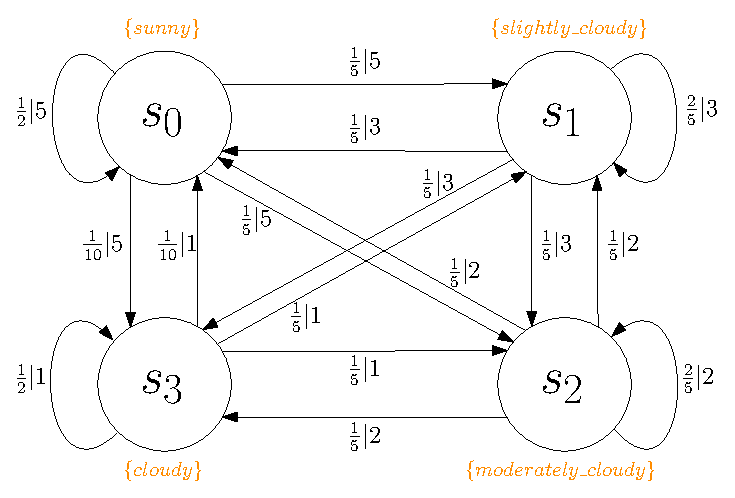
\includegraphics[width=0.6\linewidth]{resources/weather-solar-pannel}
    \caption{MC modeling a daily production of energy (in $kJ$) of solar panels according to weather}
    \label{MCexample}
  \end{figure}
  The way $w$ is defined for this MC yields that, when a day is sunny, the installation produces $5 kJ$ during this day, $3 kJ$ when a day is slightly cloudy, $2 kJ$ when a day is moderately cloudy and, finally, $1 kJ$ when the day is cloudy.
\end{example}

\subsection{Paths of Markov chains}
Before addressing how to compute probabilities in MCs, we must introduce the notion of paths in MCs. Actually, probabilistic events of MCs are sets of paths and prefixes of paths are used to generate these events.
\begin{definition}[\textbf{Paths of an MC}] Let $\mathcal{M} = (S, \Delta, w, AP, L)$ be an MC.
A \textit{path} $\pi = s_0 s_1 s_2 \dots$ of $\mathcal{M}$ is a (infinite) sequence of states of the MC such that for all $i \in \mathbb{N}$, $\Delta(s_i, s_{i+1})> 0$. We denote by $Paths(s)$ the set of paths $\pi = s_0s_1s_2\dots$ of $\mathcal{M}$ starting from the state $s \in S$, i.e., such that $s_0 = s$.
\end{definition}
\begin{definition}[\textbf{Finite paths of an MC}]
Let $\mathcal{M} = (S, \Delta, w, AP, L)$ be an MC.
A \textbf{finite} path $\hat{\pi} = s_0 \dots s_n$ of $\mathcal{M}$, with $n \in \mathbb{N}$, is a finite sequence of states of $\mathcal{M}$ such that $\Delta(s_i, s_{i+1}) > 0$ for all $i \in \{0, \dots, n-1\}$.
We denote by $Paths_{fin}(s)$ the set of finite paths $\hat{\pi} = s_0 \dots s_n$ starting from the state $s \in S$, i.e., such that $s_0 = s$
\end{definition}
\begin{definition}[\textbf{Prefixes of paths}]
Let $\mathcal{M} = (S, \Delta, w, AP, L)$ be an MC and $\pi = s_0s_1s_2 \dots$ be a path of $\mathcal{M}$. A prefix of $\pi$ is a finite path $\hat{\pi} = s'_0 \dots s'_n$, with $n \in \mathbb{N}$, such that $s'_i = s_i$ for all $i \in \{0, \dots, n\}$.
The set of all prefixes of $\pi$ is denoted by $pref(\pi)$.
\end{definition}

\subsection{Probabilities and events in Markov chains}

We are now interested in probabilistic events of MCs and how measuring them. These events can be formulated with the notion of \textit{cylinder set}.

\begin{definition}[\textbf{Cylinder set}]
Let $\mathcal{M} = (S, \Delta, w, AP, L)$ be an MC, $s \in S$ be a state of $\mathcal{M}$ and $\hat{\pi} \in Paths_{fin}(s)$ be a finite path of $\mathcal{M}$.
\[Cyl(\hat{\pi})=\{\pi\in Paths(s)\;|\;\hat{\pi}\in pref(\pi) \} \]
\end{definition}

We can express all events with this formulation. For example, the event that consists of a singleton containing just a single path $\pi = s_0s_1\dots$ is given by $\bigcap_{\hat{\pi} \in pref(\pi)} Cyl(\hat{\pi})$

\begin{theorem}\label{theo1}
  Let $\mathcal{M}=(S, \Delta, w, AP, L)$ be an MC and $s \in S$ be a state of $\mathcal{M}$. There exists a unique probability measure $\mathbb{P}_s$ on the
  $\sigma$-algebra over $Paths(s)$ where the probabilities of cylinder sets (i.e., of events) are given by
  \[
    \mathbb{P}_s(Cyl(s_0 \dots s_n)) = \prod_{i = 0}^{n - 1} \Delta(s_i, s_{i+1})
  \]
  whit $s_0 = s$ and $n \in \mathbb{N}$.
\end{theorem}
\begin{corollary}
Any event defined using complementation or countable union of cylinder sets are also measurable.
\end{corollary}

\begin{example}[\textit{Measuring an event of an MC modeling a solar panel system}]
  Let $\mathcal{M}_{sp} = (S, \Delta, w, AP, L)$ be the MC of the example \ref{solar-panel}. The probability of sunny weather four days in a row starting on a sunny day is given
  by $\mathbb{P}_{s_0}(Cyl(s_0s_0s_0s_0)) = (\frac{1}{2})^3 = \frac{1}{8}$
\end{example}

\subsection{Objectives in Markov chains}

With this background, we can now introduce some classical problems that consist
of completing an objective in an MC. The first one that we will tackle is the reachability problem.
%\subsubsection{Reachability problem}
\begin{definition}[\textbf{Reachability event}]
  Let $\mathcal{M} = (S, \Delta, w, AP, L)$ be an MC and $T \subseteq S$ be a set of target states. The event of reaching $T$, denoted by $\Diamond T$,
  is defined as a finite union of cylinder sets. Indeed, let $s \in S$ be a state of $\mathcal{M}$ and $Paths_{fin}^T(s)$ be the set of finite paths $\hat{\pi} = s_0 \dots s_n \in Paths_{fin}(s)$, such that for all $i \in \{0, \dots, n-1 \}, \, s_i \not \in T$ and $s_n \in T$,
  \[ \Diamond T = \bigcup_{s_0 \dots s_n \in Paths_{fin}^T(s)} Cyl(s_0 \dots s_n) \]
  Since all cylinders of the set $Paths_{fin}^T(s)$ are disjoint (their prefixes are different), we can measure $\Diamond T$ with:
  \[
    \mathbb{P}_s(\Diamond T) = \sum_{s_0 \dots s_n \in Paths_{fin}^T(s)}  \mathbb{P}_s(Cyl(s_0 \dots s_n))
  \]
\end{definition}
It remains to compute this probability.

\begin{theorem}
Computing $\mathbb{P}_s(\Diamond T)$ for all $s \in S$ can be done in polynomial
time through a linear equations system (cf. appendix \ref{app-reach} for more details).
\end{theorem}

% \begin{example}[\textit{Reachability property in an MC modeling a solar panel system}]
%   Let $\mathcal{M}_{sp}$ be the MC modeling the system of the example \ref{solar-panel}.
%    The probability that a cloudy day eventually comes, starting on a sunndy day, is one, i.e., $\mathbb{P}_{s_0}(\Diamond \{s_3\}) = 1$. Indeed, the underlying graph of $\mathcal{M}_{sp}$ is strongly connected, so reaching any state starting from any state has always a probability $1$.
% \end{example}

Now, we will consider the \textit{cost of paths} of an MC. Furthermore, we
are interrested by the cost of paths to reach $T$. To compute this cost, we use the \textit{truncated sum function}.

\begin{definition}[\textbf{Truncated sum}]
  Let $\mathcal{M}=(S, \Delta, w, AP, L)$ be an MC, $s \in S$ be a state of $\mathcal{M}$, $\pi = s_0s_1s_2\dots \in Paths(s)$ be a path of $\mathcal{M}$ and $T \subseteq S$ be a set of target states.
  The trunacted sum of $\pi$ is the cost to reach $T$ through $\pi$
  for the first time. More formally, the function $TS^T: Paths(s) \rightarrow \mathbb{N} \cup \{\infty\}$ is defined as follows:
	\[
		TS^T(\pi) =
		\begin{cases}
			\sum_{i = 0}^{n-1} w(s_i, s_{i+1}) & \quad \text{if } \forall i \in \{0, \dots, n - 1\}, s_i \not\in T \text{ and } s_n \in T \\
			\infty & \quad \text{else, if } \forall i \in \mathbb{N}, \, s_i \notin T
		\end{cases}
	\]
\end{definition}
With this function, it is now possible to introduce the concept of
expected cost of paths of an MC to reach a set of targets as well as
the probability of reaching this target set with a cost bounded.

\begin{definition}[\textbf{Expected cost of paths of an MC for reachablity properties}]
	Let $\mathcal{M} = (S, \Delta, w, AP, L)$ be an MC, $s \in S$ be a state of $\mathcal{M}$ and $T \subseteq S$ be a set of target states. We define the expected cost to reach $T$, i.e., $\mathbb{E}_s(\Diamond T)$, corresponding to \textit{the expected truncated sum of paths from $s$ to reach $T$} as follows:
	\begin{itemize}
	\renewcommand{\labelitemi}{\tiny$\bullet$}
	\item If $\mathbb{P}_s(\Diamond T) < 1$, then $\mathbb{E}_s(\Diamond T) = \infty$.%(par la propriété \ref{prop-ts}).
	\item Else, if $\mathbb{P}_s(\Diamond T) = 1$, then:
	\[
    \mathbb{E}_s(\Diamond T) = \sum_{c = 0}^\infty c \cdot \mathbb{P}_s(\{\pi \in Paths(s) \; | \; TS^T(\pi) = c \})
  \]
	\end{itemize}
\end{definition}

An equivalent characterisation of the expected cost from $s \in S$ to $T$ in case of $\mathbb{P}_s(\Diamond T) = 1$ is given by
\[
  \mathbb{E}_s(\Diamond T) = \sum_{\hat{\pi} \in Paths_{fin}^T(s)} \mathbb{P}_s(Cyl(\hat{\pi})) \cdot TS^T(\hat{\pi})
\]
with $Paths^T_{fin}(s)$, the set of finite paths $\hat{\pi} = s_0 \dots s_n \in Paths_{fin}(s)$  such that, for all $i \in \{0, \dots, n-1\}, s_i \not \in T$ and $s_n \in T$. Since we can measure the probability of cylinder sets of finite paths of $\hat{\pi} \in Paths_{fin}^T(s)$, we can compute $\mathbb{E}_s(\Diamond T)$.

\begin{theorem}
  Computing $\mathbb{E}_s(\Diamond T)$ for all $s \in S$ can be done in polynomial time through a linear equations system (cf. appendix \ref{app-expMC} for more details).
\end{theorem}

The last concept that we will define in MCs is the cost bounded reachability.

\begin{definition}[\textbf{Cost bounded reachability probability}]
	Let $\mathcal{M} = (S, \Delta, w, AP, L)$ be an MC, $s \in S$ be a state of $\mathcal{M}$, $T \subseteq S$ be a set of target states and $l \in \mathbb{N}$ be a length threshold.
  The \textit{probability to reach $T$ from $s$ with a cost bounded} by the threshold $l$ is defined as follows:
	\[
    \mathbb{P}_s(\Diamond_{\leq l} T) = \mathbb{P}_s(\{\pi \in Paths(s) \; | \; TS^T(\pi) \leq l \})
  \]
\end{definition}
The event $\{\pi \in Paths(s) \; | \; TS^T(\pi) \leq l \}$ is actually measurable
in the unfolded MC until $l$.
\begin{theorem}
  The probability of the cost bounded reachability to a set of target states $T \subseteq S$ from a state $s \in S$ can be computed in pseudo-polynomial time in the size of $\mathcal{M}$ and $l$, through an unfolding of $\mathcal{M}$ until $l$.
\end{theorem}

Intuitively, we unfold $\mathcal{M}$ by recording in each state the cost of
current paths. The new set of target states in the unfolded MC is the set of
target states in $\mathcal{M}$ that have a current cost less than $l$ (cf.
appendix \ref{app-cbrMC} for more details). Finally, it remains to compute the probability to
reach these new target states in the unfolded MC. \\

Now, we can define what is a Markov decision process and introduce the concept of strategy, that is the pillar concept of resolving objective problems in such models.

\section{Markov decision processes}
Markov decision processes are systems that modelise situations describing both non-deterministic and stochastic evolution. Indeed, in comparison with Markov chains, a Markov decision process requires a decision making to go from a state of the model to its successors. After that, the system evolves following the probability distribution formed by this state and the decision taken.

\begin{definition}[\textbf{Markov decision process}]
	A \textit{Markov decision process}, (denoted by \textbf{MDP}) is defined by a tuple $\mathcal{M}  = (S, A, \Delta, w, AP, L)$ where
	\begin{itemize}
		\item $S$ is a countable set of states,
		\item $A$ is a countable set of actions ; we denote by $A(s) \in 2^A$  the set of enabled actions when the system is in state $s$ such that, for all $s \in S$,
    $A(s) \neq \emptyset$,
		\item $\Delta: S \times A \times S \rightarrow [0, 1] \cap \mathbb{Q}$ is the probability transition function such that
		\begin{flalign*}
			&\forall s \in S, \; \forall \alpha \in A(s), \; \sum_{s' \in S} \Delta(s, \alpha, s') = 1 \\
			\text{and } &\forall s, s' \in S, \; \forall \alpha \in A \setminus A(s), \; \Delta(s, \alpha, s') = 0
		\end{flalign*}

			where $\Delta(s, \alpha, s')$ defines the probability of going from $s$ to $s'$ in one transition when the action $\alpha \in A(s)$ is chosen,
    \item $w: A \rightarrow \mathbb{N}_0$ %est la fonction
        %de poids associant à chaque transition un coût strictement positif.
      is a weight function that links a strictly positive cost to each action,
    \item $AP$ is a set of atomic propositions, and
    \item $L: S \rightarrow 2^{AP}$ is a labeling function.
	\end{itemize}
  \textit{Remark: }again, $AP$ and $L$ can be ommited. In that case, we consider that $AP=S$ and $L$ is the natural labeling of each state, i.e., for all state $s \in S$, $L(s) = \{s\}$.
\end{definition}

\begin{property}
  Let $\mathcal{M} = (S,A, \Delta, w, AP, L)$ be an MDP, $s \in S$ be a state of $\mathcal{M}$ and $\alpha \in A(s)$ be an enabled action of the state $s$. The transition function $\Delta$ defines a probability distribution $\Delta_{s, \alpha}: S \rightarrow \mathcal{D}(S), \, s' \mapsto \Delta(s, \alpha, s')$ on $S$.
\end{property}
\begin{property}
  An MC is essentially an MDP where, for each state $s$, $|A(s)| = 1$.
\end{property}

We will now introduce some useful notations.

\begin{notation}
  Let $\mathcal{M}=(S, A, \Delta, w, AP, L)$ be an MDP,
  \begin{itemize}
    \item $Pred(s) = \{ s' \in S \; | \; \exists \alpha \in A(s'), \, \Delta(s', \alpha, s) > 0 \}$ is the set of predecessors of the state $s \in S$ in the the MDP,
    \item $Succ(s) = \{ s' \in S \; | \; \exists \alpha \in A(s), \, \Delta(s, \alpha, s') > 0 \}$ is the set of successors of the state $s \in S$ in the MDP and
    \item $Succ(s, \alpha) = \{ s' \in S \; | \; \Delta(s, \alpha, s') > 0 \}$
      is the set of $\alpha$-successors of the state $s \in S$ in the MDP, i.e., the set of possible successors of $s$ when the action $\alpha$ is chosen
  \end{itemize}
\end{notation}

%The underlying graph of an MDP $\mathcal{M}$ is a directed graph where vertices are states of $\mathcal{M}$ and each edge starting from a state $s$ to one of its successor $s'$ exists if and only if there exists an enabled action $\alpha$
%of $s$ such that $\Delta(s, \alpha, s') > 0$. For the other elements of the tuple defining $\mathcal{M}$, the graph is essentially caracterised the same way as for an MC.
We can represent an MDP with its underlying directed graph, the same way as for an MC, with the exception that each vertex representing a state $s$ has outgoing edges to intermediate vertices representing enabled actions of $s$ and, for each enabled action $\alpha$ of $s$, edges go from the vertex representing $\alpha$ to vertices representing $\alpha$-successors of $s$.

\begin{notation}[\textit{Size of an MDP}]
  An MDP $\mathcal{M}=(S, A, \Delta, w, AP, L)$ is called \textit{finite} if its state space $S$ is finite. The size of $\mathcal{M}$ corresponds to the size
  of the set $\{(s, \alpha, s') \in S \times A \times S \; | \; \Delta(s, \alpha, s') > 0 \}$, i.e., the number of outgoing edges of vertices representing actions in the underlying graph of $\mathcal{M}$.
\end{notation}

\begin{example}\label{simple-mdp}
  Let $\mathcal{M} = (S, A, \Delta, w, AP, L)$ be the MDP of the figure \ref{mdp01}. We have that $S = \{s_0, s_1, s_2\}$, $A = \{\alpha, \beta, \gamma\}$ and $AP=\{a, b\}$. If the system currently is in state $s_0$, labeled with $L(s_0) = \{a\}$, the only action available is $\beta$ (because $A(s_0) = \{\beta\}$).
  The cost of choosing $\beta$ is $w(\beta) = 3$.
  Thus, the system evolves following the probability distribution defined by $\Delta_{s_0, \beta}$: it has a probability of $\frac{1}{2}$
  to go to its $\beta$-successor $s_1$ and a same probability to go to its $\beta$-successor $s_2$. Let assume that the system evolves to the state $s_2$, a state with no label ($L(s_2) = \emptyset$). So, in that case, the system has two possible decisions: $\alpha$ or $\gamma$ (because $A(s_2) = \{\alpha, \gamma\}$). If $\alpha$ is chosen, the system returns to $s_2$ with a probability one and a cost of $w(\alpha) = 5$. Else, if $\gamma$ is chosen, the system goes to $s_0$ with a probability one and a cost of $w(\gamma) = 2$.
  \begin{figure}[h!]
    \centering
    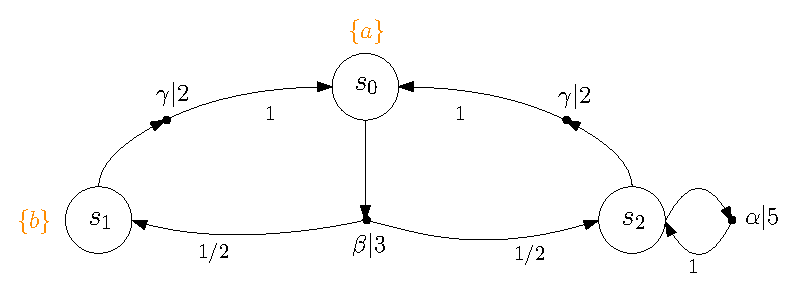
\includegraphics[width=0.7\linewidth]{resources/simple-mdp}
    \caption{MDP with $3$ states, $3$ actions and $2$ atomic propositions}\label{mdp01}
  \end{figure}
\end{example}

\subsection{Strategies in Markov decision processes}
In order to resolve nondeterminism inside MDPs, we need the notions of paths in MDPs and strategies.
\begin{definition}[\textbf{Paths in an MDP}]
  Let $\mathcal{M}=(S, A, \Delta, w, AP, L)$ be an MDP and the transition relation
  \[\rightarrow \; =  \{ (s, \alpha, s') \in S \times A \times S \; | \; \Delta(s, \alpha, s') > 0 \}, \,\]
	a path $\pi$ of $\mathcal{M}$ is defined as a sequence of states and actions
	\[ \pi = s_0 \xrightarrow{\alpha_1} s_1 \xrightarrow{\alpha_2} s_2 \xrightarrow{\alpha_3} \dots \]
	Let $s \in S$ be a state of $\mathcal{M}$, we denote by $Paths(s)$ the set of
	paths of $\mathcal{M}$ starting from the state $s$, i.e., such that $s_0 = s$.
\end{definition}
In opposition of MCs, there is no probabilistic space defined on paths of MDPs.
This is related to nondeterminism linked to the choices of possible actions when the system is in a state. We need strategies to resolve nondeterminism.
\begin{definition}[\textbf{Histories}]
	Let $\mathcal{M} = (S, A, \Delta, w, AP, L)$ be an MDP. An \textit{history} of $\mathcal{M}$
	is a finite sequence of states $(s_0 \dots s_n) \in S^+$ where, for all
	$i \in \{1, \dots, n \}, \; \exists \alpha \in A(s_{i-1})$ such that $\Delta(s_{i-1}, \alpha, s_i) > 0$.
	An history is the sequence of states that brought the state $s_0$ to the state $s_n$ along a path of $\mathcal{M}$. The set of histories of $\mathcal{M}$  is given by $\mathcal{H}(S)$.
\end{definition}

These notions allow to introduce strategies in MDPs.

\begin{definition}[\textbf{Pure strategy}]
Let $\mathcal{M} = (S, A, \Delta, w, AP, L)$ be an MDP. A \textit{strategy} (also named \textit{policy} or \textit{scheduler} in literature) for $\mathcal{M}$
	is a function
	$\sigma: \mathcal{H}(S) \rightarrow A$
	that selects, for a given history $h = (s_0 \dots s_n) \in \mathcal{H}(S)$, an enabled action of $s_n$, i.e., $\sigma(s_0 \dots s_n) = \alpha \in A(s_n)$.
	The path $\pi = s_0 \xrightarrow{\alpha_1} s_1 \xrightarrow{\alpha_2} s_2 \xrightarrow{\alpha_3} \dots$
	is a $\sigma$-path iff $\alpha_i = \sigma(s_0 \dots s_{i-1})$
	for all $i \in \mathbb{N}_0$. The set of $\sigma$-paths starting from the state $s \in S$ is given by $Paths^\sigma(s)$.
\end{definition}
Strategies that we study here are \textit{pure}, i.e., each action is chosen by strategy with probability one. We will see later that \textit{randomised} strategies exist and are essential to resolve some types of problems in MDP. \\

If a strategy controls the decisions of an MDP, then the nondeterminism is solved
and the MDP acts like an MC. Actually, an MDP $\mathcal{M}$ controlled by a strategy $\sigma$ can be formalised as an MC $\mathcal{M}^\sigma$.

\begin{definition}[\textbf{Markov chain induced by strategy}]
Let $\mathcal{M} = (S, A, \Delta, w, AP, L)$ be an MDP and $\sigma$ be a strategy for
$\mathcal{M}$. The MC induced by $\sigma$ is given by
$ \mathcal{M}^\sigma = (\mathcal{H}(S), \Delta^\sigma, w^\sigma, AP, L^\sigma) $, where, for all history
$h = s_0 s_1 \dots s_n$ of $\mathcal{M}$,
\begin{itemize}
\item $\Delta^\sigma(h, h . s_{n+1}) = \Delta(s_n, \sigma(h), s_{n+1})$
\item $w^\sigma(h, h . s_{n+1}) = w(\sigma(h))$
\item $L^\sigma(h . s_{n+1}) = L(s_{n+1})$
\end{itemize}
\end{definition}

\begin{property}
  Let $\mathcal{M}$ be an MDP, $\sigma$ be a strategy on $\mathcal{M}$ and $s\in S$ be a state of $\mathcal{M}$. There exists a bijection between the
  set $Paths^\sigma(s)$ on $\mathcal{M}$ and the set $Paths(s)$ on the MC induced by the strategy $\sigma$, $\mathcal{M}^\sigma$.
\end{property}

Since events of an MC is measurable, events of an MDP controlled by strategy is also measurable.
\begin{notation}
  We denote by $\mathbb{P}_s^\sigma$ the probability measure defined on paths starting from the state $s$ of the Markov chain induced by the strategy $\sigma$.
\end{notation}

Markov chains induced by such (infinite memory) strategies can be seen as forests of trees representing an infinite unfolding of the MDP where actions are controlled by strategy (this is due to the fact that the set of histories of an MDP is infinite). So, such induced MCs have infinite size. Actually, such strategies are not easy to use in practice because it requires to
know the complete history of the system to decide which action to choose. \textit{Finite memory strategies} allow to avoid this problem.

\begin{definition}[\textbf{Finite memory strategy}]
Let $\mathcal{M} = (S, A, \Delta, AP, L)$ be an MDP.
A \textit{finite memory strategy} $\sigma = (Q, \sigma_\alpha, \delta, \delta_0)$ is a \textit{Moore machine} where
\begin{itemize}
	\item $Q$ is a finite set of \textit{modes},
	\item $\sigma_\alpha: Q \times S \rightarrow A$ is a function that chooses, for any $s \in S$, an action $\alpha \in A(s)$ following a mode $q \in Q$ in which the machine currently is,
	\item $\delta: Q \times S \rightarrow Q$ is the transition function,
	\item $\delta_0: S \rightarrow Q$ is the function that chooses the initial mode of the machine following a state $s \in S$ of the MDP from which the machine is initialised.
\end{itemize}
\end{definition}

\begin{definition}[\textbf{Product of an MDP by a strategy}]
Let $\mathcal{M} = (S, A, \Delta, w, AP, L)$ be an MDP and $\sigma = (Q, \sigma_\alpha, \delta, \delta_0)$ be a finite memory strategy for $\mathcal{M}$.
The product of $\mathcal{M}$ by $\sigma$ is given by
\[ \mathcal{M} \times \sigma = \mathcal{M}^\sigma = (S \times Q, \Delta^\sigma, w^\sigma, AP, L^\sigma) \]
where $\mathcal{M}^\sigma$ is the MC induced by the finite memory strategy $\sigma$ and where,
for all states $s, s' \in S$ and for all modes $q, q' \in Q$ of the strategy,
\begin{itemize}
	\item $\Delta^\sigma((s, q), (s', q')) =
	\begin{cases}
	\Delta(s, \sigma_\alpha(q, s), s') & \text{if } \delta(q, s) = q'\\
	0  & \text{else}
	\end{cases}$
  \item $w^\sigma((s, q), (s', q')) = w(\sigma_\alpha(q, s))$
  \item $L^\sigma(s, q) = L(s)$
\end{itemize}
\end{definition}

\begin{example}[\textit{Product of an MDP by a strategy}]
  Let $\mathcal{M}=(S, A, \Delta, w, AP, L)$ be the MDP of the example \ref{simple-mdp} and $\sigma = (Q, \sigma_\alpha, \delta, \delta_0)$ be the
  finite memory strategy of the figure \ref{finite_mem_strat}.
  \begin{figure}[h!]
    \centering
    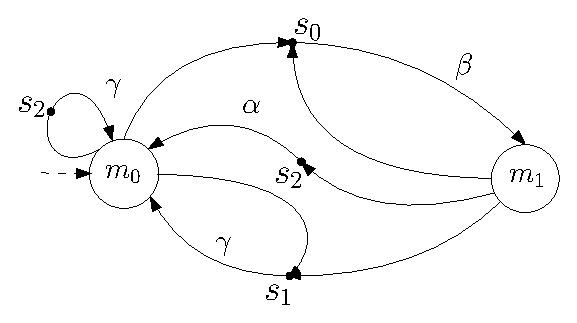
\includegraphics[width=0.4\linewidth]{resources/strategy}
    \caption{Finite memory strategy for $\mathcal{M}$ with $2$ modes}\label{finite_mem_strat}
  \end{figure}

  We assume that, for all $s \in S$, $\delta_0(s) = m_0$. The strategy simply consists in choosing once $\alpha$ when the system enters in the state $s_2$ and choosing $\gamma$ just after that, to return to $s_0$. The MC induced by the product of $\mathcal{M}$ by $\sigma$ is given in the figure
  \ref{inducedMC}.
  \begin{figure}[H]
    \centering
    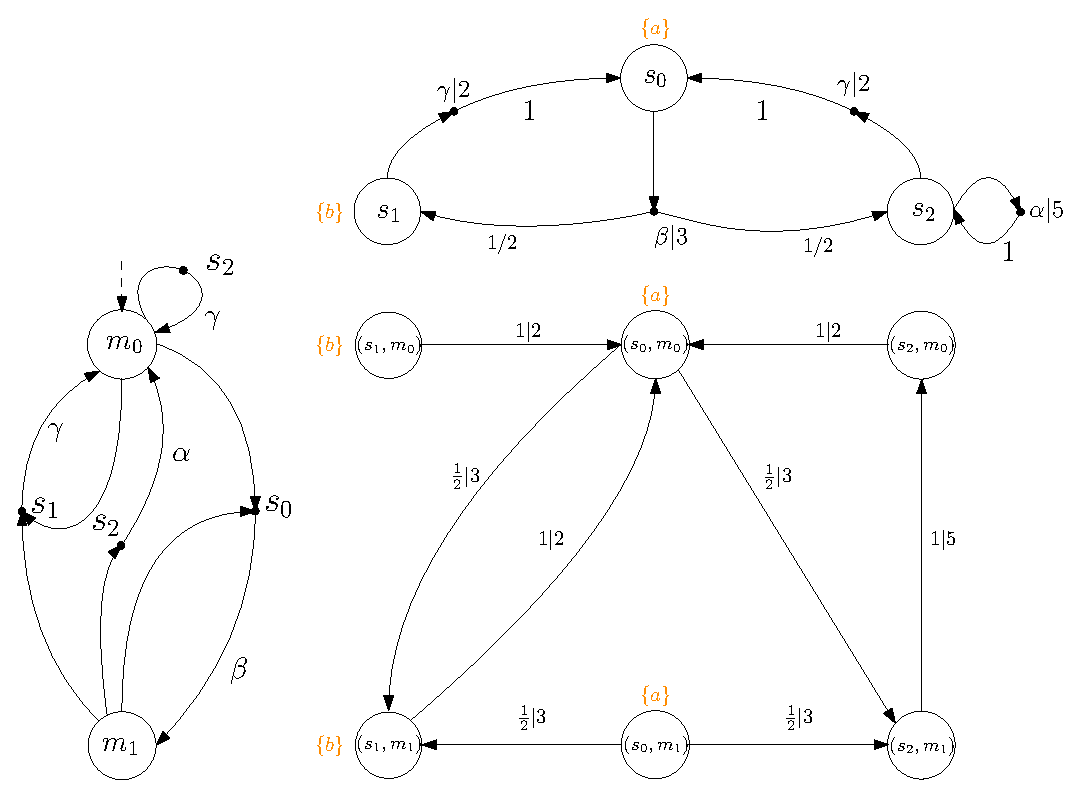
\includegraphics[width=0.55\linewidth]{resources/inductedmarkov}
    \caption{Product of $\mathcal{M}$ by $\sigma$}\label{inducedMC}
  \end{figure}
\end{example}

Finally, the last type of strategy that we will see is a particular case of finite memory strategies, where strategies have only one mode.
In that case, the action chosen by a such strategy only depends on the current state of the system.

\begin{definition}[\textbf{Memoryless strategy}]
  Let $\mathcal{M}=(S, A, \Delta, w, AP, L)$ be an MDP. A \textit{memoryless strategy} is a function
  $
    \sigma: S \rightarrow A
  $ that links each state $s$ of $\mathcal{M}$ to an enabled action $\alpha \in A(s)$ of this state.
\end{definition}

\begin{property}
  A memoryless strategy is a finite memory strategy with only one mode.
\end{property}

\subsection{Objectives in Markov decision processes}
The resolution of problems in MDPs will be done through strategies that will choose the optimal actions to complete different objectives. As for MCs, we will first address the \textit{stochastic reachability problem} in an MDP.
\begin{definition}[\textbf{SR problem}]
  Let $\mathcal{M}=(S, A, \Delta, w, AP, L)$ be an MDP, $s \in S$ be a state of $\mathcal{M}$, $T$ be a set of target states and $\alpha \in [0, 1]$ be
  a probability threshold. The \textit{stochastic reachability} (SR) problem consists
  of deciding if a strategy $\sigma$ exists such that
  \[
    \mathbb{P}_s^\sigma(\Diamond T) \geq \alpha
  \]
\end{definition}

\begin{theorem}
  The SR-problem can be decided in polynomial time in the size of $\mathcal{M}$
  through a linear program, by building a pure memoryless strategy that gives the optimal actions to reach $T$ from every state $s \in S$ (cf. appendix \ref{app-sr} for more details).
\end{theorem}

Before introducing the following, we will first introduce the \textit{truncated sum} of paths of MDPs in order to compute the cost of paths of an MDP.

\begin{definition}[\textbf{Truncated sum for MDPs}]
	Let $\mathcal{M} = (S, A, \Delta, w, AP, L)$ be an MDP, $s \in S$ be a state of $\mathcal{M}$, $T \subseteq S$ be a set of target states and
	$\pi = s_0 \xrightarrow{\alpha_1} s_1 \xrightarrow{\alpha_2} s_2 \xrightarrow{\alpha_3} \dots \in Paths(s)$ be a path of
	$\mathcal{M}$ starting from $s$. The truncated sum $TS^T: Paths(s)
	\rightarrow \mathbb{N} \cup {\infty}$ of the path $\pi$ is defined as follows:
	\[
		TS^T(\pi) =
		\begin{cases}
			\sum_{i = 1}^{n} w(\alpha_i) & \quad \text{if } \forall i \in \{0, \dots, n - 1\}, s_i \notin T \text{ and } s_n \in T \\
			\infty & \quad \text{else, if $ \forall i \in \mathbb{N}, \, s_i \not\in T$}
		\end{cases}
	\]

\end{definition}

By considering the cost of paths of an MDP, we are now interested by building
strategies inducing the shortest path to go from one state to a set of target
states. The notion of shortest path in an MDP is not as obvious as in a graph due to the uncertainty linked to the stochastic environment.
The stochastic shortest path problem in an MDP can be approached in different
ways. We will first approach the \textit{stochastic shortest path expectation} problem and
then approach the \textit{stochastic shortest path percentile} problem. \\

Since events of any MDP controlled by strategy is measurable and
since the cost of paths of any MDP is computable via the truncated sum function, we can
compute the expected length of paths that reach a set of target states using a strategy and, more particularly, build the strategy that will minimise the expected length of these paths.

\begin{definition}[\textbf{SSP-E problem}]
Let $\mathcal{M}=(S, A, \Delta, w, AP, L)$ be an MDP, $s \in S$ be a state of $\mathcal{M}$,
$T \subseteq S$ be a set of target states and $l \in \mathbb{N}$ be a paths length
threshold. The \textit{stochastic shortest path expectation} (SSP-E) problem
consists of deciding if a strategy $\sigma$ exists such that
\[
  \mathbb{E}^\sigma_s(\Diamond T) \leq l
\]
% i.e., if there exists a strategy $\sigma$ such that the expected length of paths starting in the state $s$ in the MC induced by this strategy is lower than the length threshold $l$.
where $\mathbb{E}_s^\sigma(\Diamond T)$ corresponds to the expected cost of paths starting from $s$ in the MC induced by $\sigma$.
\end{definition}

\begin{theorem}
  The SSP-E problem can be decided in polynomial time in the size of $\mathcal{M}$, through a linear program by building a pure memoryless strategy that gives the optimal actions to minimise the expected cost of paths to reach $T$ from every state $s \in S$ (cf. appendix \ref{app-sspe} for more details).
\end{theorem}

Finally, the last problem that we will present in this chapter is the
\textit{stochastic shortest path percentile} problem. For this problem, we will
be interested to decide if there exists a strategy that allows to reach a set of target states with
a cost bounded and an high probability threshold.

\begin{definition}[\textbf{SSP-P problem}]
  Let $\mathcal{M} = (S, A, \Delta, w, AP, L)$ be an MDP, $s \in S$ be a state of
  $\mathcal{M}$, $T \subseteq S$ be a set of target states, $l \in \mathbb{N}$
  be a paths length threshold and $\alpha \in [0, 1]$ be a probability
  threshold. The \textit{stochastic shortest path percentile} (SSP-P) problem
  consists of deciding if there exists a strategy $\sigma$ such that
  \[
    \mathbb{P}_s^\sigma (\Diamond_{\leq l} T) \geq \alpha
  \]
\end{definition}

\begin{theorem}
  The SSP-P problem can be decided in pseudo-polynomial time in the size of $\mathcal{M}$ and $l$ by building a pure finite memory strategy. This strategy is built by unfolding the MDP $\mathcal{M}$ from the state $s$ until $l$ and by resolving the SR problem on this unfolded MDP.
\end{theorem}

\begin{definition}[\textbf{Unfolded MDP until a bounded length}] Let
  $\mathcal{M} = (S, A, \Delta, w, AP, L)$ be an MDP, $s^* \in S$ be a state of
  $\mathcal{M}$, $T \subseteq S$ be a set of target states of $\mathcal{M}$ and $l \in \mathbb{N}$ be a paths length threshold.
  Unfolding $\mathcal{M}$ from $s^*$ until $l$ can be done as follows: \\
  We build $\mathcal{M}_l = (S_l, A_l, \Delta_l, w, AP, L_l)$ for the subset $T_l \subseteq S_l$ where
  \begin{itemize}
  \item $S_l$ is composed of states $(s, v)$ where $s \in S$ et $v \in \{0, \dots, l\} \cup \{\bot\}$.
  We consider that $\bot > l$, with $\bot + v = \bot$ for all $v \in \{0, \dots, l\}$.
  Intuitively, $v$ records the cost of paths while unfolding $\mathcal{M}$.
  As we unfold $\mathcal{M}$ from $s^*$, we have that
  $(s, 0) \not \in S_l$ for all $s \in S$ such that $s \neq s^*$.
  \item For each $\alpha \in A$, we have that $\alpha \in A_l$ and for all $(s, v) \in S_l$, $A_l(s, v) = A(s)$.
  \item $\Delta_l: S_l \times S_l \rightarrow [0, 1]$ is the probability transition function given by:\\
  $\text{Forall } (s, v), (s', v') \in S_l \text{ and for all } \alpha \in A(s),$
  \[
  \Delta_l((s, v), \alpha, (s', v')) =
  \begin{cases}
  	\Delta(s, \alpha, s') & \quad \quad \text{ if } v' = v + w(\alpha) \leq l \text{ or}\\
  	 & \quad \quad \text{ if } v' = \perp \text{ and } v+w(\alpha) > l \\
  	0 & \quad \quad \text{ else}
  \end{cases}
  \]
  \item $L_l:S_l \rightarrow AP \mapsto L_l((s, v)) = L(s)$.
  \item Target states are states of
  $T_l = \{(s, v) \;|\; s \in T \wedge v \leq l \}$.
  \end{itemize}
  \textit{Remark}: since all state $(s, v) \in S_l$ such that $v = \bot$ can never reach $T_l$, it is not useful to keep these states in the unfolded MDP $\mathcal{M}_l$. So, we can replace all these states in $S_l$ with a unique state $\bot$ such that, for all $(s, v) \in S_l$ such that $v \neq \bot$ and for all $\alpha \in A(s)$ such that $v + w(\alpha) > l$,
  $\Delta_l((s, v), \alpha, \bot) = 1$. Then, we define a new action $\alpha_\bot \in A_l$ with an arbitrary weight that will allow a self-loop for $\bot$, i.e., $\Delta_l(\bot, \alpha_\bot, \bot)=1$.
\end{definition}

\begin{example}[\textit{Unfold an MDP}]
  Let $\mathcal{M} = (S, A, \Delta, w, AP, L)$ be the MDP of the example \ref{simple-mdp}.
  This MDP can be unfolded from the state $s_0$ until the threshold $l = 8$ for the target states set $\{s_1\}$ (cf. figure \ref{unfolding}).
  \begin{figure}[h!]
    \centering
    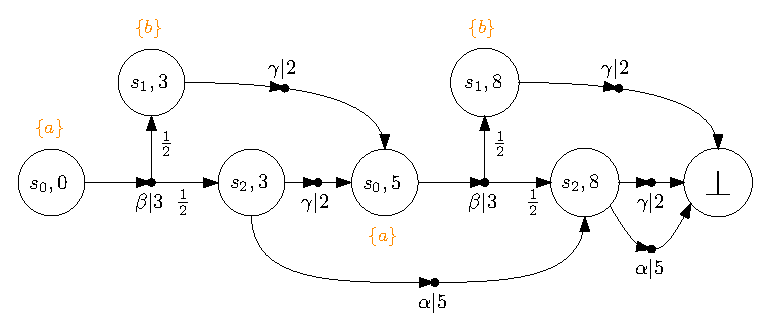
\includegraphics[width=0.8\linewidth]{resources/unfolding}
    \caption{$\mathcal{M}$ unfolded from $s_0$ until $l=8$ for $\{s_1\}$}\label{unfolding}
  \end{figure}
  The highlighted strategy in the figure \ref{unfolding} is the memoryless strategy that resolves the SR problem in $\mathcal{M}_l$. This strategy is the
  same as the one that resolves the SSP-P problem in $\mathcal{M}$ and is thus finite memory in $\mathcal{M}$.
\end{example}


\bibliographystyle{plain}
\bibliography{bib}

\chapter*{Appendix}
\addcontentsline{toc}{chapter}{Appendix}
\markboth{Appendix}{Appendix}
\stepcounter{chapter}

\section{Linear equations systems}
\subsection{Reachability in a MC}
Let $\mathcal{M} = (S, \Delta, w, AP, L)$ be a MC, $s \in S$ be a state of $\mathcal{M}$ and $T \subseteq S$ be a set of target states in $\mathcal{M}$.
We can compute the probability to reach $T$ from $s$ :
let $(x_s)_{s \in S}$ be a vector of probabilities,
\begin{itemize}
	\item if $s$ is not connected to $T$ in the underlying graph of $\mathcal{M}$, then we have $x_s = 0$
	\item else, if $s \in T$, then we obviously have $x_s = 1$
	\item else, for all $s \in S \setminus T$  such that $s$ is connected to $T$ in the underlying graph of $\mathcal{M}$,
		\[
      x_s = \underbrace{\sum_{s' \in S \setminus T} \Delta(s, s') \cdot x_{s'}}_{\text{reach $T$ via $s' \in S \setminus T$}} + \underbrace{\sum_{t \in T} \Delta(s, t)}_{\text{reach $T$ in one transition}}
    \]
\end{itemize}
This defines a linear equations system.
Let $S_{=0}$ be te subset of states of $S$ that can not reach $T$ in the underlying graph of $\mathcal{M}$, $S_{=1} = T$ and $S_{=?} = S \setminus (S_{=0} \cup S_{=1})$.
The solution $(x_s)_{s \in S_{=?}}$ of this linear equations system is unique and $x_s = \mathbb{P}_s(\Diamond T)$ for all $s \in S$.

\subsection{Expected cost of paths of a MC for reachability properties}
  Let $\mathcal{M} = (S, \Delta, w, AP, L)$ be a MC, $s \in S$ be a state of $\mathcal{M}$ and $T \subseteq$ S be a set of targets states. $\mathbb{E}_s(\Diamond T)$ can be computed through a linear equations system defined as follow :
  %Soient $x_s = \mathbb{E}_s(TS^T)$ %et $S_{=1} = \{s \in S \; | \; \mathbb{P}_s_s(\Diamond T) = 1 \}$
  let $succ(s) = \{ s' \in S \; | \; \Delta(s, s') > 0 \}$ be the set of successors of $s$,
  \[ x_s =
  	\begin{cases}
  	\infty & \quad \text{if } \mathbb{P}_s(\Diamond T) < 1 \\
  	0 & \quad \text{if } s \in T \\
  	\sum_{s' \in succ(s)} \Delta(s, s') \cdot (w(s, s') + x_{s'}) & \quad \text{else}
  	\end{cases}
  \]
Let $S_{=?} = \{ s \in S \; | \; \mathbb{P}_s(\Diamond T) = 1 \} \setminus T$. The solution $(x_s)_{s \in S_{=?}}$ of this linear equations system is unique and $x_s = \mathbb{E}_s(\Diamond T)$ for all $s \in S$.

\section{Cost bounded reachability in a MC}

Let $\mathcal{M} = (S, \Delta, w, AP, L)$ be a MC. We denote by $\mathbb{P}^\mathcal{M}_s$ the probability measure $\mathbb{P}_s$ such that $s \in S$ is a state of the MC $\mathcal{M}$.
Let $s \in S$ be a state of $\mathcal{M}$, $T \subseteq S$ be a set of target states and $l \in \mathbb{N}$, a threshold.
We can compute $\mathbb{P}_s(\Diamond_{\leq l} T)$ by reduction to the reachability problem on $\mathcal{M}_l = (S_l, \Delta_l)$ to the target states set $T_l \subseteq S_l$ that we build as follow :
\begin{itemize}
	\item $S_l$ is composed of states $(s, v)$ such that $s \in S $ and $v \in \mathbb{N} \cup \{ \bot \}$. We consider that $\bot > l$, with $\bot + v = \bot$ for all $v \in \mathbb{N}$. Intuitively, we record in $v$ the cost of paths in $\mathcal{M}$. Target states are states of $T_l = \{ (s, v) \in S_l \; | \; s \in T \wedge v \leq l \}$.
	\item $\Delta_l: S_l \times S_l \rightarrow [0,1]$ is the probability transition function given by:\\
	$\forall (s, v), (s', v') \in S_l,$
	\[
		\Delta_l((s, v), (s', v')) =
		\begin{cases}
		\Delta(s, s') & \text{if $v' = v + w(s, s')$ and $v' \leq b$  or} \\
		 & \text{if $v' = \bot$ and $v + w(s, s') > b$} \\
		 0 & \text{else}
		\end{cases}
	\]
\end{itemize}
\textit{Note} : here, the weight function is ommited in $\mathcal{M}_l$. So, $\mathcal{M}_l$ is unweighted. \\
Resolving the cost bounded reachability by the threshold $l$ from $s$ to $T$ in $\mathcal{M}$ can be done by resolving the reachbility problem from $(s, 0)$ to $T_l$ in $\mathcal{M}_l$, i.e., $\mathbb{P}^\mathcal{M}_s(\Diamond_{\leq l} T) = \mathbb{P}^{\mathcal{M}_l}_{(s, 0)}(\Diamond T_l)$

\section{Linear programs}
\subsection{SR problem}
Let $\mathcal{M}=(S, A, \Delta, w, AP, L)$ be a MC and $T \subseteq S$ be a set of target states of $\mathcal{M}$. We will resolve the SR problem by building the strategy $\sigma$ that will maximise the
probability of reaching $T$ from all $s \in S$. Let $s \in S$ be a state of $\mathcal{M}$ and $\alpha \in [0, 1]$ be a probability threshold. If $\mathbb{P}_s^\sigma(\Diamond T) \geq \alpha$, $\sigma$ obviously resolves the
SR problem. Otherwise, no strategy exist to solve the SR problem. So, we will first compute $\mathbb{P}_s^{\max}(\Diamond T)$ for all $s \in S$. Let $(x_s)_{s \in S}$
be a probability vector for the following LP :
\[
	\min \sum_{s \in S} x_s
\]
under the constraints :
\begin{flalign*}
	x_s &= 1 \quad &&\forall s \in T, \\
	x_s &= 0 \quad &&\forall s \not\in T \text{ such that $s$ is not connected to $T$ in $G^\mathcal{M}$}, \\
	x_s &\geq \sum_{s' \in S} \Delta(s, \alpha, s') \cdot x_{s'}
	\quad &&\forall \alpha \in A(s) \text{ and } \forall s \not \in T \text{ such
		that $s$ is connected to $T$ in $G^\mathcal{M}$}. \\
	0 &\leq x_s \leq 1 && \forall s \in S
\end{flalign*}
\textit{Note : we denote by $G^\mathcal{M}$ the underlying graph of $\mathcal{M}$}. \\

The optimal solution $(v_s)_{s \in S}$ of this LP is unique and gives the following result :
\[
	v_s = \mathbb{P}_s^{\max}(\Diamond T) \quad \forall s \in S
\]
From this result, we can build a memoryless strategy $\sigma$ such that
$\mathbb{P}^\sigma_s(\Diamond T) = \mathbb{P}^{\max}_s(\Diamond T)$.
To do that, for each state $s$, we build $A^{\max}(s)$, the set of
actions $\alpha \in A(s)$ such that
$
	v_s = \sum_{s' \in S} \Delta(s, \alpha, s') \cdot v_{s'}
$. So, as we have $v_s = \mathbb{P}^{\max}_s(\Diamond T)$, actions of $A^{\max}(s)$
maximise the probability of reaching $T$ from $s$.
Building a strategy that would arbitrarely choose a state from
$A^{\max}(s)$ is not sufficient. Indeed, if we take a state $s$
such that $A^{\max}(s) = \{\alpha, \beta\}$ where $\Delta(s, \beta, t) = 1$
for a certain $t \in T$ and $\Delta(s, \alpha, s) = 1$, we obviously have
that choosing $\alpha$ doesn't allow to reach $T$ passing by $s$.
\\

A selection of action that ensures
the reachability of $T$ in the
MC induced by $\sigma$ is required.
Let $\mathcal{M}^{\max}$ be the MDP that corresponds to $\mathcal{M}$
where the actions $\beta \in A(s) \setminus A^{\max}(s)$ are deleted from $A(s)$
for all $s$ connected to $T$.
By definition, $\mathbb{P}^{\max}_s(\Diamond T)$ is not affected by this simplification of
$\mathcal{M}$. \\

For all $s$ such that $s$ is connected to $T$ in the underlying graph of
$\mathcal{M}^{\max}$, we denote by $||s||$ the length of the \textit{shortest path} of $s$ to any state of $T$ in the underlying graph of
$\mathcal{M^{\max}}$. Intuitively, computing $||s||$ allow to avoid that $\sigma$ chooses
actions that prevent $s$ of reaching $T$.
\begin{itemize}
	\renewcommand{\labelitemi}{\tiny$\bullet$}
	\item $||s|| = 0$ iff $s \in T$.
	\item Let $n \in \mathbb{N}_0$. By induction on $n$, we define
		$\sigma(s)$ for each $s$ connected to $T$ in the underlying graph of
		$\mathcal{M^{\max}}$ and such that $||s|| = n$.
		The strategy chooses an action $\sigma(s) \in A^{\max}(s)$ such that there exists $s' \in Succ(s, \sigma(s))$ where $\Delta(s, \sigma(s), s') > 0$, with $s'$ connected to $T$ in the underlying graph of
		$\mathcal{M}^{\max}$ and $||s'|| = n - 1$. An action $\sigma(s) \in A(s)$ is chosen
		arbitrarely for states $s$ that are not connected to $T$ in the underlying graph of $\mathcal{M}$.
\end{itemize}
We build $\sigma$ this way : let $s \in S$ be a state of $\mathcal{M}$ and $\mathbb{A}(s) = \{\alpha \in A^{\max}(s) \; | \; \exists s' \in Succ(s,
	\alpha), \, ||s'|| = ||s|| - 1 \}$,
\[
	\sigma(s) = \arg \max_{\alpha \in \mathbb{A}(s)} \sum_{s' \in Succ(s, \alpha)} \Delta(s,
	\alpha, s') \cdot v_{s'}
\]

\subsection{SSP-E problem}
Let $\mathcal{M}=(S, A, \Delta, w, AP, L)$ be a MC and $T \subseteq S$ be a set
of target states of $\mathcal{M}$. We will resolve the SSP-E problem by building a strategy $\sigma$ that will minimise the expected cost of paths to reach $T$
from all $s \in S$. Let $s \in S$ be a state of $\mathcal{M}$ and $l \in \mathbb{N}$ be a length threshold. If $\mathbb{E}_s^\sigma(\Diamond T) \geq l$, $\sigma$ obviously resolves the
SSP-E problem. Otherwise, no strategy exist to solve the SSP-E problem. So, we will first compute $\mathbb{E}^{\min}_s(\Diamond T)$ for all $s \in S$.
Let $S_{=1} = \{ s \in S \; | \; \mathbb{P}^{\max}_s(\Diamond T) = 1 \}$ be the set of states that reach $T$ with a maximum probability one and $(x_s)_{s \in S}$ be a costs vector for the following LP :
		\[ \max \sum_{s \in S_{=1}} x_s \]
		under the constraints \\
	%	\begin{equation*}
	%  \renewcommand{\arraystretch}{1.3}
	%  \begin{array}{ll}
	%		x_s = \infty \quad
	%	\end{array}
	%\end{equation*}
	\begin{flalign*}
		x_s &= 0 && \forall s \in T \\
		x_s &= \infty && \text{$\forall s \in S$ such that $\mathbb{P}^{\max}_s(\Diamond T) < 1$} \\
		x_s &\leq w(\alpha) + \sum_{s' \in S \setminus T} \Delta(s, \alpha, s')
			\cdot x_{s'} && \forall \alpha \in A(s) \text{ and } \forall s \in S \setminus T \text{ such that } \mathbb{P}^{\max}_s(\Diamond T) = 1
	\end{flalign*}
The optimal solution $(v_s)_{s \in S}$ of this LP is unique and gives the following result :
\[
	v_s = \mathbb{E}^{\min}_s(\Diamond T) \quad \forall s \in S
\]
We can now build an optimal pure memoryless strategy $\sigma$ that minimises the expected cost of paths of $\mathcal{M}$ to reach $T$ :
\begin{align*}
	\sigma(s) = \arg \min_{\alpha \in A(s)} ( w(\alpha) &+
		\sum_{s' \in S \setminus T} \Delta(s, \alpha, s') \cdot v_{s'} ) \\
	\text{and }
	\mathbb{E}^\sigma_s(\Diamond T) &= \min_\sigma \mathbb{E}^\sigma_s(\Diamond T)
\end{align*}

\end{document}
